\documentclass{report}
% \renewcommand{\thesection}{\arabic{section}}
\setcounter{tocdepth}{1}
% index
\usepackage{imakeidx}
\makeindex%[title=Index, intoc]
% glossary
% \usepackage{glossaries}
% \makeglossaries
% geometry formatting
\usepackage{authblk}
\usepackage[utf8]{inputenc}
\usepackage[margin=0.625in]{geometry}
\usepackage{parskip, setspace}
\setstretch{1.5}
% math formatting
\usepackage{amsmath, amsfonts}
% \numberwithin{equation}{section}
% code formatting
\usepackage{listings}
\usepackage{xcolor}

\definecolor{codegreen}{rgb}{0,0.6,0}
\definecolor{codegray}{rgb}{0.5,0.5,0.5}
\definecolor{codepurple}{rgb}{0.58,0,0.82}
\definecolor{backcolour}{rgb}{0.75,0.75,0.75}

\lstdefinestyle{mystyle}{
    backgroundcolor=\color{backcolour},   
    commentstyle=\color{codegreen},
    keywordstyle=\color{red},
    numberstyle=\tiny\color{codegray},
    stringstyle=\color{codepurple},
    basicstyle=\ttfamily\footnotesize,
    breakatwhitespace=false,         
    breaklines=true,                 
    captionpos=b,                    
    keepspaces=true,                 
    numbers=left,                    
    numbersep=5pt,                  
    showspaces=false,                
    showstringspaces=false,
    showtabs=false,                  
    tabsize=4
}

\lstset{style=mystyle}
% rich text
\usepackage{graphicx, caption, wrapfig}
\usepackage{hyperref}
% bibliography
\usepackage{biblatex}
\addbibresource{bib.bib}

% \renewcommand{\arraystretch}{1.5} % give a little more space in table

\title{CS 530: High-Performance Computing \\ Seminar 1: A Survey of Computational Physics}
\author{Nathan Chapman}
\affil{Department of Computer Science \\ Central Washington University}
\date{\today}

\begin{document}

\maketitle

\tableofcontents

% \listoffigures

% \chapter{Introduction}

%     % \begin{itemize}
%     %     \item There are really hard and complex problems that are reasonably solved by hand
%     %     \item There are problems with no analytic solution
%     %     \item There are really big problems that require high-performance computing
%     %     \item Computational physics lies at the intersection of Math, Physics, and Computer Science
%     %     \item The difference between ``doing physics on the computer'' and ``computational physics'' is the consideration of numerical analysis
%     % \end{itemize}

% \chapter{Mathematical Methods}

%     \chapter{Taylor Series}

%     \chapter{Fourier Analysis}

%         \section{Fourier Series}

%         \section{The Fourier Transform}

%     \chapter{Properties of Differential Equations}

%         \section{Order}

%         \section{Linearity}

%         \section{Homogeneity}

%         \section{Chaos \& Entropy}

%             \subsection{Poincar{\'e} Sections}

%     \chapter{Ordinary Differential Equations}

%     \chapter{Partial Differential Equations}

%         \section{Parabolic PDEs}

%             \subsection{The Heat Equation}

%         \section{Hyperbolic PDEs}

%             \subsection{The Wave Equation}

%         \section{Sturm-Liouville Theory}

%         \section{Green's Functions}

%     \chapter{Differential Equations with Conditions}

%         \section{Initial Conditions}

%         \section{Boundary Conditions}

%             % \begin{itemize}
%             %     \item Dirichlet
%             %     \item Neumann
%             %     \item Robin
%             %     \item Mixed
%             %     \item Cauchy
%             % \end{itemize}

%     \chapter{Systems of Differential Equations}

%         \section{Coupled Systems}

%     \chapter{Eigenvalue Problems}

%     \chapter{Optimization}

% \chapter{Computational Methods}

%     \chapter{Programming Language}

%         \section{Fortran}

%         \section{Julia}

%         \section{Python}

%         \section{Matlab \& Mathematica}

%     \chapter{Finite-Differences}

%         \section{Order}

%         \section{Accuracy}

%     \chapter{Runge-Kutta Methods}

%     \chapter{Symplectic Integrators}

%     \chapter{Parareal - Parallel-in-Time Integration}

%     \chapter{The Fast Fourier Transform}

%         \section{FFTW}

%             \subsection{CUDA FFTW}

%     \chapter{Finite-Element Methods}

%     \chapter{Markov Chains \& Monte-Carlo Methods}

% \chapter{Physical Context}

%     \chapter{Orbital Dynamics}

%         \section{The N-Body Problem}

%     \chapter{Fluid Dynamics}

%         \section{The Lattice Boltzmann Method}

%     \chapter{Electrodynamics \& Magnetohydrodynamics}

%         \section{Fringing Electric Fields of Non-Ideal Capacitors}

%     \chapter{Many-Body Quantum Mechanics}

%         \section{Quadrupole-Quadrupole Interactions in a BEC}

%     \chapter{Numerical Relativity}

%         \section{Mercury's Perihelion Shift}

%             \subsection{Effects of Eccentricity}

%             \subsection{Gravitational Wave Chirp}

%         \section{Gravitational Waves}

%     \chapter{Chaotic Systems}

%         \section{Atmospheric Physics}

%         \section{Forced Oscillators}

%     \chapter{Honorable Mentions}

%         \section{Projectile Motion with Drag}

% \chapter{Numerical Analysis}
    
%     \chapter{Error}

%     \chapter{Lax Equivalence Theorem}

%     \chapter{Courant-Friedrichs-Lewy condition}

%     \chapter{Von Neumann Stability}

%     \chapter{Energy Drift}

%     \chapter{Stiff Differential Equations}

%     \chapter{Grids \& Meshes}

%     \chapter{Numerical Diffusion}

\chapter{Introduction}

    Each of the five pillars of physics (Classical Mechanics\index{Mechanics}\index{Mechanics!Classical}, Electromagnetism\index{Electromagnetism}, Relativity\index{Relativity}, Quantum Mechanics\index{Mechanics!Quantum}, and Thermodynamics\index{Thermodynamics}) has well-posed problems for which the mathematical models are either unreasonable or impossible to solve by hand.  As such, computational methods are needed to get an approximate solution.  
    
    There are many numerical methods to support the evolution of physical models for each domain.  Whether it be using a fourth-order Runge-Kutta\index{Runge-Kutta} method to solve the first-order ordinary differential equation \index{Differential Equation!Ordinary} that models a ballistic object under the influence of gravity and air-resistance, or using an eigth-order symplectic\index{Symplectic} Yoshida integrator\index{Integrator!Symplectic} to model a system of bodies orbiting each other while accounting for the produced gravitational waves, there are methods for every physical context.  Though, because these methods are using approximations to their analytic counterparts in calculus, there is error that needs to be considered.

    Numerical analysis\index{Numerical Analysis} is the practice of tracking and rigorously accounting for the discrepancies that arise when approximating analytic mathematical methods by their finite and counterparts.  These errors can arise not only from approximating descriptions from calculus, but also from operations in linear algebra as they're applied to finding the eigenvalues of quantum operators.

\chapter{Classical Mechanics} \label{sec:classical}

    The ``everyday'' world as we know it is described by a model of physics that has been studied for millenia.  As such, we call this model of the behavior of nature ``Classical Mechanics''\index{Mechanics!Classical}.  Now I hear you ask ``Why?''.  Well ``mechanics''\index{Mechanics} is the study of motion, and we include the ``classical'' preface to distinguish it from ``modern'' physics which encompasses all the physics discovered after around 1905 or 1925 (depending on who you ask); those physics will be covered later in sections \ref{sec:quantum} and \ref{sec:relativity}.  For now we take a look at the mathematical model that describes the motion of not-too-small, not-too-large objects moving at slow velocities.
    
    The motion of ``classical'' objects, ranging in scale from biological cells, sand, ants, birds, cars, airplanes, planets, up to stars, can described as the solution to what's called the \emph{equation of motion}\index{Equation of Motion}.  The equation of motion for an object with mass $m$ under the influence of forces $F_i$ is determined by Newton's 2nd law of motion\index{Newton!2nd Law}
    
    \begin{equation} \label{eq:newton}
        \sum_i \mathbf{F}_i = m \ddot{\mathbf{x}},
    \end{equation}

    where $\ddot{\mathbf{x}}$ represents the second time derivative\index{Derivative} of the position\index{Position} $\mathbf{x}$ known as \emph{acceleration}\index{Acceleration}.  These forces completely determine the how objects move through space in time.
    
    Mathematically, the resulting equation is a vector second-order ordinary differential equation\index{Differential Equation!Second Order}, compactly representing the underlying system of differential equations\index{Differential Equation!System}.  In many cases, this differential equation is homogenous\index{Differential Equation!Homogenous} to represent no time-dependent external forces supplying the physical system with energy\index{Energy}.  Likewise, sometimes these forces can be represented by nonlinear\index{Nonlinear} terms; making the equation of motion much more complex.
    
    The following is a survey of topics in classical mechanics whose forces yield an equation of motion either too complex or too unreasonable to solve by hand.

\pagebreak

    \section{N-Body Orbits} \label{subsec:orbits}

        While so-called N-Body\index{N-Body} problems are prolific in physics and other sciences, a quintessential example is the gravitational\index{Gravity} interaction of astrophysical bodies i.e. massive bodies in space.

        \subsection{Mathematical Model: Systems of Ordinary Differential Equations}

            In the case of multi-body gravitaitonal interactions, the governing equation of motion\index{Equation of Motion} is determined via Newton's law of gravitation\index{Newton!Gravitation} between two objects with masses $m_i$ and $m_j$

            \begin{equation}
                F_{ij} = \frac{G m_i m_j}{r_{ij}^2} \hat{r}
            \end{equation}

            where $G = 6.67 \times 10^{-11} \frac{N m^2}{kg^2}$ is the universal gravitaional constant, $r_{ij}$ is the distance between the two objects, and $\hat{r}$ is the unit vector pointing from object $i$ toward $j$.  Not only are is there an equation of motion for each object, but each equation is coupled to every other equation.  This results in the three-dimensional vector differential equation\index{Differential Equation}\cite{taylor2005classical}

            \begin{equation}
                \sum_{j; i \neq j} \frac{G m_i m_j}{(x_i - x_j)^2 + (y_i - y_j)^2 + (z_i - z_j)^2} \frac{(x_j - x_i) \hat{x} + (y_j - y_i) \hat{y} + (z_j - z_i) \hat{z}}{\sqrt{(x_i - x_j)^2 + (y_i - y_j)^2 + (z_i - z_j)^2}} = m_i (\ddot{x_i} \hat{x} + \ddot{y_i} \hat{y} + \ddot{z_i} \hat{z})
            \end{equation}

            for object $i$, and a similar equation for every other object.  For example, a system of 3 objects interacting only via gravitational forces has the equations of motion 

            \begin{align}
                \frac{G m_2}{((x_1 - x_2)^2 + (y_1 - y_2)^2 + (z_1 - z_2)^2)^{3/2}} 
                \begin{bmatrix}
                    x_2 - x_1 \\
                    y_2 - y_1 \\
                    z_2 - z_1
                \end{bmatrix} + 
                \frac{G m_3}{((x_1 - x_3)^2 + (y_1 - y_3)^2 + (z_1 - z_3)^2)^{3/2}} 
                \begin{bmatrix}
                    x_3 - x_1 \\
                    y_3 - y_1 \\
                    z_3 - z_1
                \end{bmatrix} &= \begin{bmatrix}
                    \ddot{x_1} \\
                    \ddot{y_1} \\ 
                    \ddot{z_1}
                \end{bmatrix} \\
                %
                \frac{G m_1}{((x_2 - x_1)^2 + (y_2 - y_1)^2 + (z_2 - z_1)^2)^{3/2}} 
                \begin{bmatrix}
                    x_1 - x_2 \\
                    y_1 - y_2 \\
                    z_1 - z_2
                \end{bmatrix} + 
                \frac{G m_3}{((x_2 - x_3)^2 + (y_2 - y_3)^2 + (z_2 - z_3)^2)^{3/2}} 
                \begin{bmatrix}
                    x_3 - x_2 \\
                    y_3 - y_2 \\
                    z_3 - z_2
                \end{bmatrix} &= \begin{bmatrix}
                    \ddot{x_2} \\
                    \ddot{y_2} \\ 
                    \ddot{z_2}
                \end{bmatrix} \\
                %
                \frac{G m_1}{((x_3 - x_1)^2 + (y_3 - y_1)^2 + (z_3 - z_1)^2)^{3/2}} 
                \begin{bmatrix}
                    x_1 - x_3 \\
                    y_1 - y_3 \\
                    z_1 - z_3
                \end{bmatrix} + 
                \frac{G m_2}{((x_3 - x_2)^2 + (y_3 - y_2)^2 + (z_3 - z_2)^2)^{3/2}} 
                \begin{bmatrix}
                    x_2 - x_3 \\
                    y_2 - y_3 \\
                    z_2 - z_3
                \end{bmatrix} &= \begin{bmatrix}
                    \ddot{x_3} \\
                    \ddot{y_3} \\ 
                    \ddot{z_3}
                \end{bmatrix}
            \end{align}

            Because this problem is in three dimensions, there are actually 9 differential equations to solve in order to fully model the evolution of the position\index{Position} and velocity\index{Velocity} over time of each object.

        \subsection{Computational Model}
        
            \subsubsection{Finite Differences}

                Because computers can only store numbers of finite precision, approximations must be used in order to implement these differntial equations in a form that can be understood by the computer.  One such translation is by approximating the analytic derivatives and differential operators with \emph{finite differences}\index{Finite Differences}. In its most basic form, the derivative\index{Derivative} can be approximated as a ratio of differences in the form

                \begin{equation}
                    \frac{df}{dt} \approx \frac{f(t + \Delta t) - f(t)}{\Delta t}.
                \end{equation}

                This equation is known as the first-order-accurate\index{Finite Differences!First Order}, forward-finite-difference\index{Finite Differences!Forward} representation of the first-order derivative\index{Derivative!First Order} \textbf{[NEEDS CITATION]}.  There are similar representations for higher-order derivatives, more accurate approximations, and more accurate approximations of higher-order derivatives. Similarly, there are also \emph{central}\index{Finite Differences!Central} and \emph{backward}\index{Finite Differences!Backward} finite-differences.

                Each of these finite-difference schemes can be represented via coefficients\index{Finite Differences!Coefficients}.  For example, the derivative of order $m$\index{Derivative!Order} with accuracy $n$\index{Finite Differences!Accuracy} has $2p + 1 = 2 \lfloor \frac{m + 1}{2} \rfloor - 1 + n$ central\index{Finite Differences!Central} coefficients $a_{-p}, a_{-p + 1}, \ldots, a_{p - 1}, a_p$ defined such that

                \begin{equation}
                    \begin{bmatrix}
                        1         & 1             & \ldots & 1            & 1 \\
                        -p        & -p + 1        & \ldots & p - 1        & p \\
                        (-p)^2    & (-p + 1)^2    & \ldots & (p - 1)^2    & p^2 \\
                        \vdots    & \vdots        & \vdots & \vdots       & \vdots \\
                        (-p)^{2p} & (-p + 1)^{2p} & \ldots & (p - 1)^{2p} & p^{2p} 
                    \end{bmatrix}
                    \begin{bmatrix}
                        a_{-p} \\
                        a_{-p + 1} \\
                        \vdots \\
                        \vdots \\
                        a_p
                    \end{bmatrix} = 
                    \begin{bmatrix}
                        0 \\
                        \vdots \\
                        m! \\
                        \vdots \\
                        0
                    \end{bmatrix}
                \end{equation}

                where the only non-zero value on the right side of the equation is at the $m+1$-th index\textbf{[NEEDS CITATION]}.
                
                Once the derivative\index{Derivative} operators are discretized\index{Discretize} using finite-differences\index{Finite Differences}, there are different algorithms in which the differences are used to solve the differential equations\index{Differential Equation}.

            \subsubsection{Symplectic Integrators}

                While there are many methods of numerically solving differential equations\index{Differential Equation} (known as \emph{integrators}\index{Integrator}), one of the most important classes when considering a context such as orbital mechanics\index{Mechanics} and oscillatory\index{Oscillatory} situations (i.e. Hamiltonian\index{Hamiltonian} systems) is that of \emph{symplectic} integrators\index{Integrator!Symplectic}.  This type of integrator is so important to computational physics because it conserves energy\index{Energy!Conservation} throughout time\index{Time} \textbf{[NEEDS CITATION]}.  Without energy conservation\index{Energy!Conservation}, the system becomes unphysical, which can lead to unnatural behavior such as a mass\index{Mass} on a spring\index{Spring} extending to infinity.  Two of the simplest symplectic integrators\index{Integrator!Symplectic} are the \emph{Semi-implicit Euler Method}\index{Euler}\index{Implicit}\textbf{[NEEDS CITATION]}

                \begin{subequations} \label{eq:semiEuler}
                    \begin{equation}
                        v_{n+1} = v_n + a_n \Delta t
                    \end{equation}
                    \begin{equation}
                        x_{n + 1} = x_n + v_{n+1} \Delta t
                    \end{equation}
                \end{subequations}

                and the \emph{Velocity Verlet Algorithm}\index{Velocity}\index{Verlet}\textbf{[NEEDS CITATION]}

                \begin{subequations} \label{eq:verlet}
                    \begin{equation}
                        v_{n+1} = v_n + \frac{a_n + a_{n+1}}{2} \Delta t
                    \end{equation}
                    \begin{equation}
                        x_{n + 1} = x_n + v_{n} \Delta t + \frac{1}{2} a_n \Delta t^2
                    \end{equation}
                \end{subequations}

                The velocity-Verlet algorithm in C[NEEDS CITATION TO ALGORITHM ARCHIVE]:

                

            \subsubsection{Parallel Computing}

                Because there are so many terms and equations, and each term is only needs the current step, this problem naturally lends itself to being parallelized\cite{parallelnbody}\index{Parallel}.

        \subsection{Numerical Analysis}

            \subsubsection{Discretization}

                Error\index{Error} associated with the size of the time-step\index{Step!Time} is dictated by which specific finite-difference\index{Finite Differences} method is chosen.

            \subsubsection{Energy Drift}

                In the case of orbital mechanics\index{Mechanics}, there is no loss of mechanical energy\index{Energy} (ignoring the effects of general relativity; more on this later in section \ref{sec:relativity}).  Therefore, a constraint is imposed on the system that the total mechanical energy\index{Energy} (kinetic energy + potential energy) of the system must remain constant at each point in time\index{Time}.  When using non-symplectic\index{Integrator!Symplectic} methods, this constraint is not adhered to which leads to \emph{energy drift}\index{Energy!Drift}.

\pagebreak

    \section{Fluid Dynamics}

        Fluid dynamics is 

        \subsection{Mathematical Model}

            \begin{itemize}
                \item Navier-Stokes
            \end{itemize}

        \subsection{Computational Tools}

            lattice boltzmann method in parallel and on GPU

        \subsection{Numerical Analysis}

            NS is a PDE so CFL

\pagebreak

    \section{Projectile Motion with Drag}

        Projectile motion is a fundamental concept in introductory physics as it allows students to learn how to work with problems involving forces and motion in multiple dimensions.  These considerations always neglect air-resistance, also known as \emph{drag}\index{Drag}.  This simplification is done to not only highlight the fundamentals of motion, but also because including even low-order drag terms greatly increases the complexity of the equation of motion.

        \subsection{Mathematical Model}

            Beginning again from Newton's second law\index{Newton!2nd Law} as described with equation (\ref{eq:newton}), we can fully determine the motion of an object under the influence of gravity and both linear and quadratic drag as\cite{taylor2005classical}

            \begin{subequations}
                \begin{equation}
                    m \mathbf{g} - b \left|\left| \dot{\mathbf{r}} \right|\right| \hat{\dot{r}} - c \left|\left|\dot{\mathbf{r}}\right|\right|^2 \hat{r} = m \ddot{\mathbf{r}}
                \end{equation}
                \begin{equation}
                    ||\mathbf{v}|| \hat{v} = \mathbf{v} \implies m \mathbf{g} - b \dot{\mathbf{r}} - c \left|\left|\dot{\mathbf{r}}\right|\right| \dot{\mathbf{r}} = m \ddot{\mathbf{r}}
                \end{equation}
            \end{subequations}

            where $b, c$ are physical constants determined by the geometry of the object and the medium in which it is moving, $\mathbf{g}$ is the acceleration of gravity near the surface of Earth (i.e. where the air is).  Because this equation cannot be represented as the application of a differential operator on a function or vector of functions, this equation of motion is a \emph{nonlinear} differential equation\index{Differential Equation!Nonlinear}.  In fact, because this is again a vector equation, there are actually three nonlinear differential equations that, due to the magnitude of the velocity, all rely on each other; thus this differential equation is said to be a \emph{coupled system}\index{Differential Equation!Coupled} of differential equations.  Expanded out, the equation of motion becomes the system of equations

            \begin{subequations}
                \begin{equation}
                    - b \dot{r}_x - c \sqrt{\dot{r}_x^2 + \dot{r}_y^2} \ \dot{r}_x = m \ddot{r}_x
                \end{equation}
                \begin{equation}
                    m g - b \dot{r}_y - c \sqrt{\dot{r}_x^2 + \dot{r}_y^2} \ \dot{r}_y = m \ddot{r}_y.
                \end{equation}
            \end{subequations}

        \subsection{Computational Tools}

            Just like with orbital mechanics, finite differences can be used to discretize\index{discretize} the differential equation.

        \subsection{Numerical Analysis}

\chapter{Electromagnetism}

\pagebreak

    \section{Fringing Electric Fields of Non-Ideal Capacitors}

            The following is taken from previous work\cite{fringingfieldsBealeChapman2019}.

        \subsection{Mathematical Model}

            The behavior of the electric field strength in a parallel plate capacitor can be well understood simply using the classical electromagnetism equation $E = \Delta V / d$ where $V$ is the potential difference between the two parallel plates of the capacitor and $d$ is the distance between them. However, this assumes the plates are infinitely large and ``close'' together.  A consequence of this assumption is a constant electric field between the plates and far from the edge in the finite case. We will be exploring the \emph{fringing field}, or the field that exists outside the area between the capacitors and close to the edges.

            While the fringing field is extremely difficult to model analytically, we can make use of the fact that the electric field is proportional to the gradient of the electric potential.  Since the electric potential is smooth, we can consider the electric potential at any point being the average of the electric potential of it's surrounding points. This is a simplified explanation, but as it turns out we can use this idea to model the potential field numerically.

        \subsection{Computational Tools}

            We model the electric potential of a parallel plate capacitor in a grounded box with the \emph{relaxation method} and via the \emph{Gauss-Seidel} (GS) implementation
        
            \begin{equation} \label{eq:GS}
                V_{new}[i,j]=\frac{1}{4}(V_{old}[i+1,j] +V_{new}[i-1,j]+V_{old}[i,j+1]+V_{new}).
            \end{equation}
            
            To strive for maximum computational efficiency, we augment the GS method with a \emph{Simultaneous Over-Relaxation} (SOR) as well. Our SOR method is implemented by augmenting the new potential as 
            
            \begin{equation} \label{eq:SOR}
                V_{new}[i,j]=\alpha \Delta V +V_{old}[i,j],
            \end{equation}
            
            where $\alpha$ is the relaxation coefficient defined by $\alpha = 2 / (1+ \pi / L)$, and $\Delta V$ is the difference between the new value of the potential and the old one.  With the inclusion of SOR, our computation time decreases by a factor of $L$ when compared to not including SOR.  Though, since this implementation is done numerically, several parameters of the system must be stipulated beforehand.
            
            First we will model our parallel plate capacitors to have a potential difference of $2 V$ (our left capacitor will be $1 V$ and our right will be $-1 V$), and we will place it in a grounded box of length $L$.  The size of the box, or correspondingly the size of the capacitor, are natural length scales for the problem and one can be defined in terms of the other.
            
            As a preliminary step in simulating the system numerically, we must discretize our region into cells of side length $\Delta x$.  To make sure our simulation is at least somewhat accurate, $\Delta x$ should be significantly smaller than the total side length of the grounded/bounding box. This will allow us to assign values of the electric potential to actual areas in the box.  This reassignment, from initial ``best guess'', takes the form of the GS method, shown in Equation \ref{eq:GS}.

            Now that we have a method to determine the potential of a point based on surrounding points, we will need to apply it to our model of the physical system. We will need each 'cell' to have an initial value to use our method, and so we will make an 'initial guess' for all cells that are not part of the boundary conditions. In our case we used an initial guess of $0$ for every point except the capacitors. 
            
            To find a reasonable value for the potential at each point we will need to define convergence criteria to compare against in each iteration of the averaging loop.  This is necessary because after the first round of averaging only the cells bordering the capacitors will have any change at all. The more averages we do, the more cells begin being affected by this relaxation method. Once the outermost cells are being affected, the cells closest to the capacitors have gone through many iterations of the average, and so they are more close to the true value than the outer cells. Therefore we defined convergence criteria, forcing our code to continue running through the averages and recalculating the potential until the $\Delta V$, or the difference in the potential value before and after going through the most recent round of averaging, is less than our convergence criteria, which we set to $10^{-5}$. As the cells closer to the capacitors will reach a point of small $\Delta V$ before outer cells will, we have defined our program such that it will continue running until our \textit{maximum} $\Delta V$ is less than our convergence criteria.
            
            Now that we have a complete distribution of the electric potential in our system, we can take the negative gradient of the potential to find the electric field at each point.  Though, since we're working in a discrete space, we need to rethink about how we take derivatives.

            \begin{figure}[t]
                \centering
                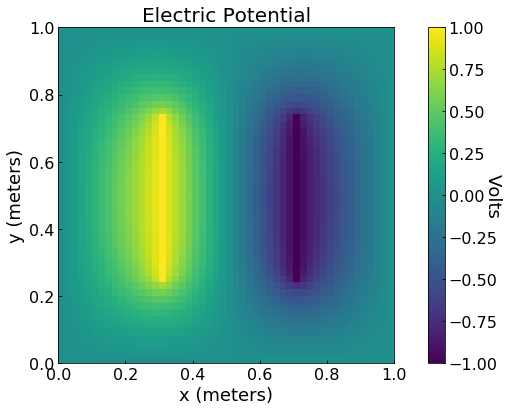
\includegraphics[width=0.45\linewidth]{images/PotentialField.png}
                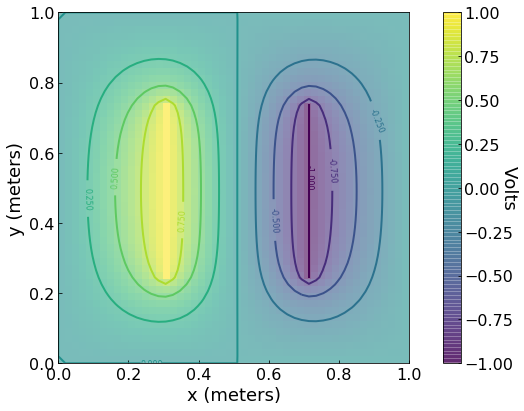
\includegraphics[width=0.45\linewidth]{images/PotentialFieldEquipotentials.png}
                \caption{The electric potential caused by capacitor, whose plates are held at a potential difference of $V=2$, with a boundary condition of $V=0$ at the edges of the box. The left plot shows only the color mapping of the potential while the bottom superimposes equipotential lines separated by $0.25 V$ each on top of the color mapping. The initial guess used for the unknown areas was $0 V$ and the convergence criteria was $10^{-5}$. The box/system is $1 \mathrm{m} \times 1 \mathrm{m}$, while the cell size is $\frac{1}{50^2} \ \mathrm{m^2}$. The separation of the capacitors is 0.4 m and it's length is 0.5 m.}
                \label{fig:PotentialField}
            \end{figure}
            
            To calculate the electric field we will consider a change in potential over a distance, which can be done with the equation
            
            \begin{equation} \label{eq:efieldcomponents}
                \begin{split}
                    E_x &=-\frac{1}{2}\left(\frac{V[i+1,j]-V[i-1,j]}{\Delta x}\right) \\
                    E_y &=-\frac{1}{2}\left(\frac{V[i,j+1]-V[i,j-1]}{\Delta x}\right).
                \end{split}
            \end{equation}
            
            These components can be used to not only show the vector field, but also to give the \emph{magnitude} of the electric field at each point.  The magnitude of the electric field at each point is then the norm of the electric field vectors at the respective points.

            Using the computational methods described in Sec. \ref{sec:Theory}, we created a plot of the potential field within our range. In Figure \ref{fig:PotentialField} we are able to observe the potential across our space. As expected our potential is highest at our left capacitor, with a voltage of +1 V, and lowest at our right capacitor, with a voltage of -1 V. Our boundary conditions at the edge also appear to be near/at zero which is to be expected. 
        
            By looking at the second plot in Figure \ref{fig:PotentialField} we can see that the electric field in between the two capacitors should be fairly constant, which is to be expected as that is the point of capacitors. 
            
            Using Equations \ref{eq:efieldcomponents}, we were able to calculate an electric field for each cell and plot them in a vector plot, shown in Figure \ref{fig:ElectricField}. The electric field looks much like we would expect it to. As we can see in the bottom plot, the electric field vectors are perpendicular to the equipotential lines, which attests to the physical accuracy of of our model. The electric field behaves like we would expect it would, with the fringing field being weaker than the field between the capacitors. The field between the capacitors is relatively constant, which is what we would hope for. We see that there is the highest magnitude electric field right around the edges of the capacitors, which makes sense as that is where the potential will be changing the fastest from the potential of the capacitor to the ground value of the edges.
            
            \begin{figure}[h]
                \centering
                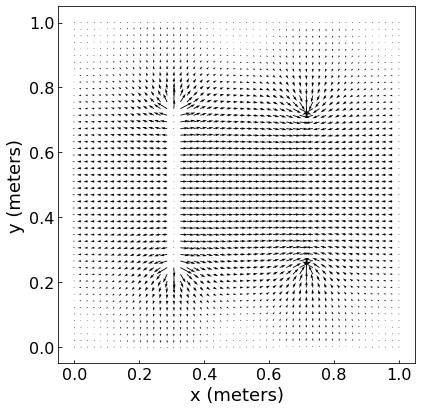
\includegraphics[width=0.27\linewidth]{images/ElectricField.png}
                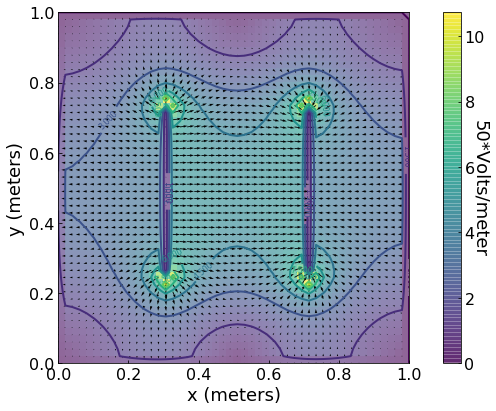
\includegraphics[width=0.32\linewidth]{images/ElectricFieldMagnitude.png}
                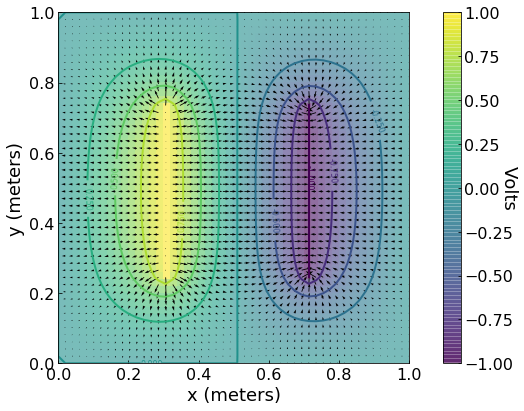
\includegraphics[width=0.34\linewidth]{images/ElectricFieldWithPotential.png}
                \caption{(Left) Electric field in the area of interest. (Center) The top plot shows the electric field vectors on their own, which the second superimposes a color map on top that represents the magnitude of the electric field in $\frac{\text{V}}{\frac{1}{50}\text{m}}$, or 50V/m. The third plot superimposes our potential field on top of the electric field lines. Variables used are the same as in Figure \ref{fig:PotentialField}.}
                \label{fig:ElectricField}
            \end{figure}
            
        \subsection{Numerical Analysis}

            As a final test of the physical accuracy of our model, we chose a spot directly centered between the two capacitors and observed how the electric field at this point changed as the separation of capacitors changed. We did this because for an ideal capacitor we can calculate the electric field simply by using Equation \ref{eq:efield}.
            
            By using both the numerical and analytical solutions shown in Figure \ref{fig:compare} we can conclude that our model seems to be more accurate for smaller seperations and increase in error as the plates get further apart. 
            
            As we can see in Figure \ref{fig:compare}, the error increases as the capacitor separation increases, which makes sense if we look back to how we need more iterations of our Gauss-Streisel SOR method to reach cells that are further away from our boundary conditions. This means that the cell in the center that we are observing has probably only recently met the convergence criteria and so is more prone to error than those that continued to be averaged long past meeting the convergence criteria. 
            
            This also makes sense physically as Equation \ref{eq:efield} assumes a perfect capacitor, which true capacitors will not have perfectly constant electric fields.
            
            As we can explain the error physically and it is small, we can use it as a model for our system.
            
            Finally we observed how cell size affected our results for the electric field. 
            
            The trend shows that as cell size is decreased it trends towards lower percent error in the electric field magnitude and thus towards a numerical convergence. We are not quite sure what the bump near 0.03 cell size means and could not identify a physical or numerical cause. As the rest of the points seems to follow a trend, we chose to make the assumption that the point was inconsistent and do not address it further.

            \begin{figure}[t]
                \centering
                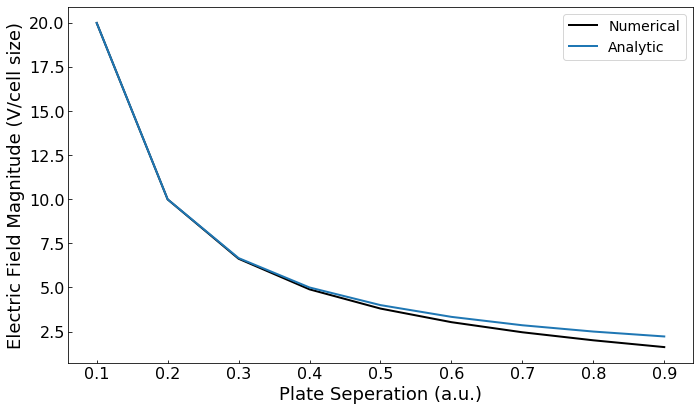
\includegraphics[width=0.48\linewidth]{images/NumericalAnalytic.png}
                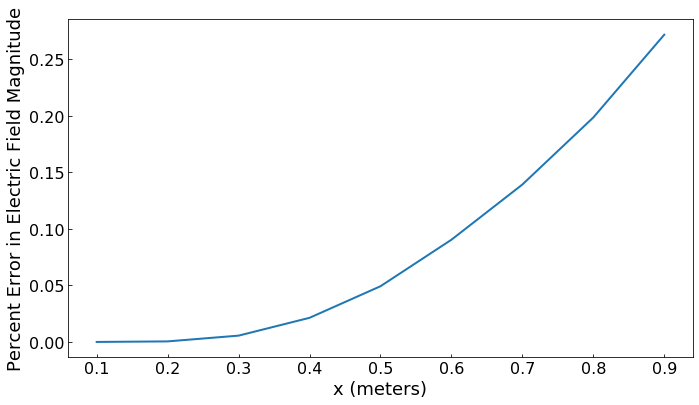
\includegraphics[width=0.49\linewidth]{images/PercentErrorSep.png}
                \caption{The top plot shows the analytic and numerical solution for the electric field magnitude directly between the parallel plate capacitors while the bottom one shows the percent error as a function of plate separation. Other than the varied plate separation, all variables used are the same as used in Figure \ref{fig:PotentialField}.}
                \label{fig:compare}
            \end{figure}
            
            Having confirmed the physical validity of our model, we proceeded to investigate how the fringing field varied with respect to plate separation and distance from capacitor.
        
            As we can see from the plots of the electric field in Figure \ref{fig:ElectricField}, the electric field is strongest at the corners of the capacitor and in between the capacitors and gets weaker as we move further away, into the fringing fields. 
            
            As for the dependence on distance between the capacitors, we were able to plot the electric field for a chosen point outside the capacitors and plot it as a function of changing separation, shown in Figure \ref{fig:sep}.
            
            \begin{figure}[h]
                \centering
                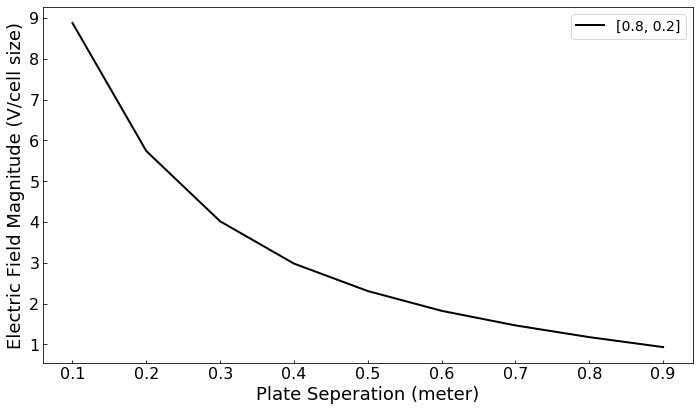
\includegraphics[width=0.66\linewidth]{images/FringeChangingSep.png}
                \caption{The numerically calculated electric field magnitude is plotted above as a function of the separation between the capacitors.}
                \label{fig:sep}
            \end{figure}
            
            In this figure, we can observe that the electric field magnitude at a spot that is 0.5 meters across the cell horizontally and 0.2 meters down from the top ground boundary condition decreases as the plate separation increases.
        
            Our model for the fringing electric field around a capacitor has created a system that seems physically reliable, as shown through it's similarity to the numerical solution in Figure \ref{fig:compare} and when evaluating cell size. Our model has allowed us to observe the fringing field for varying separations and distances from the capacitor. 
            
            Our model is limited in the resolution to which we can model the system, i.e. how small the cell size can be, due to computational time. We used a cell size of 1/50 m for all of our plots except when we were varying cell size and this achieved a resolution that was relatively smooth and resulted in enough data points to evaluate it's accuracy, as shown in Figure \ref{fig:compare}. If we made the cell size smaller, we would get smoother plots of the electric field magnitude and could model the relation to changing variables a bit more accurately, but as we had to calculate so many points for each plot the computation time took significantly longer than the added resolution was worth.
            
            Finally, we saw a weird 'bump' in our plot of the percent error in Figure \ref{fig:cellsize} which interrupted what seemed to be a fairly smooth trend. We were unable to identify the cause of the bump, but as it was small and seemed to still trend towards lower values overall, we are comfortable saying that the percent error in the electric field magnitude decreases with decreasing cell size.

            \begin{figure}[h]
                \centering
                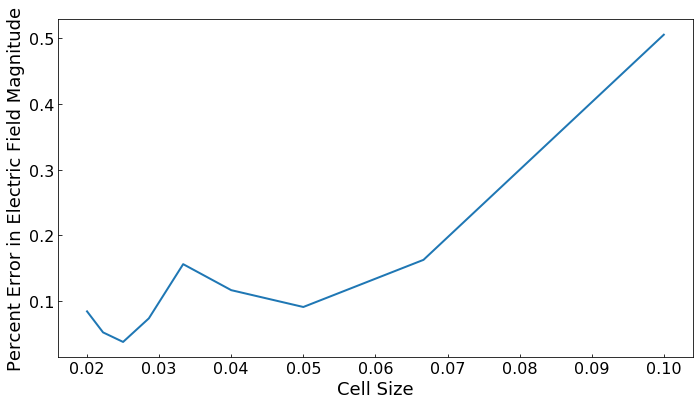
\includegraphics[width=0.66\linewidth]{images/PercentErrorCell.png}
                \caption{The percent error in the Electric Field when using the cell size of 0.01 m as a baseline. Other than varying cell size, all variables used are the same as in Figure \ref{fig:PotentialField}.}
                \label{fig:cellsize}
            \end{figure}

\pagebreak

    \section{Antenna Radiation Patterns}

        \subsection{Mathematical Model}

            In a more general setting, modelling how the electric and magnetic fields change in time and space requires the solutions to \emph{Maxwell's Equations}\index{Maxwell's Equations}\cite{griffiths2017introduction}, succinctly represented as

            \begin{equation}
            \begin{aligned}
                \nabla \cdot \mathbf{E}  &= \frac{\rho}{\epsilon_0}                 & \nabla \cdot \mathbf{B}  &= 0 \\
                \nabla \times \mathbf{E} &= -\frac{\partial \mathbf{B}}{\partial t} & \nabla \times \mathbf{B} &= \mu_0 \mathbf{J} + \mu_0 \epsilon_0 \frac{\partial \mathbf{E}}{\partial t}.
            \end{aligned}
            \end{equation}

            where $\mathbf{E}, \mathbf{B}, \mathbf{J}$

            Expanded, these equations take the form

            \begin{equation}
            \begin{aligned}
                \partial_x E_x(t, \mathbf{r}) + \partial_y E_y(t, \mathbf{r}) + \partial_z E_z(t, \mathbf{r}) &= \frac{\rho}{\epsilon_0}                 & \partial_x B_x(t, \mathbf{r}) + \partial_y B_y(t, \mathbf{r}) + \partial_z B_z(t, \mathbf{r})  &= 0 \\
                \begin{bmatrix}
                    \partial_y E_z - \partial_z E_y \\
                    \partial_z E_x - \partial_x E_z \\
                    \partial_x E_y - \partial_y E_x \\
                \end{bmatrix} &= -\partial_t \begin{bmatrix} B_x \\ B_y \\ B_z \end{bmatrix} & \begin{bmatrix}
                    \partial_y B_z - \partial_z B_y \\
                    \partial_z B_x - \partial_x B_z \\
                    \partial_x B_y - \partial_y B_x \\
                \end{bmatrix} &= \mu_0 \rho \begin{bmatrix} v_x \\ v_y \\ v_z \end{bmatrix} + \mu_0 \epsilon_0 \partial_t \begin{bmatrix} E_x \\ E_y \\ E_z \end{bmatrix}.
            \end{aligned}
            \end{equation}

            In their expanded form, Maxwell's equations form a coupled\index{Differential Equation!Coupled} system\index{Differential Equation!System} of eight \emph{partial} differential equations\index{Differential Equations!Partial} (i.e. differential equations whose solutions depend on more than one variable).  Because each of these equations must be solved simultaneously, modelling the dynamics of the electromagnetic field throughout space is quite challenging.

        \subsection{Computational Tools}

            Finite-difference time-domain

        \subsection{Numerical Analysis}

            \begin{itemize}
                \item 
            \end{itemize}

\chapter{Quantum Mechanics} \label{sec:quantum}

    \section{Quantum Chemistry}

        \subsection{Mathematical Model}

            \begin{itemize}
                \item The Schr{\"o}dinger Equation
                \item The Many-Body Schr{\"o}dinger Equation
            \end{itemize}

        \subsection{Computational Tools}

        \subsection{Numerical Analysis}

    \section{Quadrupole-Quadrupole Interactions in a BEC}

        \subsection{Mathematical Model}

            \begin{itemize}
                \item The Schr{\"o}dinger Equation
                \item The Many-Body Schr{\"o}dinger Equation
            \end{itemize}

        \subsection{Computational Tools}

        \subsection{Numerical Analysis}

\chapter{Relativity} \label{sec:relativity}

    \section{Effects of Eccentricity on Mercury's Perihelion Shift}

        \subsection{Mathematical Model}

        \subsection{Computational Tools}

        \subsection{Numerical Analysis}

    \section{Mercury's Gravitational Wave Chirp}

        \subsection{Mathematical Model}

        \subsection{Computational Tools}

        \subsection{Numerical Analysis}

    \section{Strong-Field General Relativity}

        \subsection{Mathematical Model}

        \subsection{Computational Tools}

        \subsection{Numerical Analysis}

\chapter{Conclusion}

\printbibliography

\printindex

\end{document}